\section{Συμπεράσματα}
\begin{frame}
	\frametitle{Συμπεράσματα}
	\vspace{-\baselineskip}
	\begin{center}
		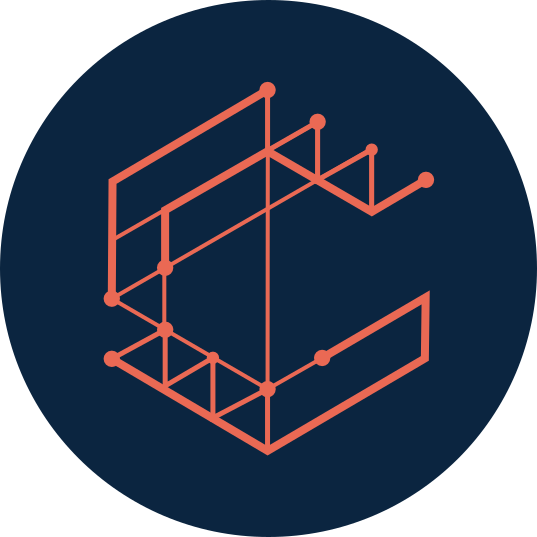
\includegraphics[width=.1\paperwidth]{assets/figures/concordia-logo}
	\end{center}
	\textbf{Concordia} - μία πλήρως αποκεντρωμένη αυτόνομη κοινωνική πλατφόρμα ...με ορισμένα εμπόδια:
	\begin{itemize}
		\item Πρώιμες τεχνολογίες
		\item Ethereum - τέλη συναλλαγών, συγκράτηση χρηστών, κλιμακοθετησιμότητα
		\item IPFS υβριδικό ως προς την ανακάλυψη κόμβων
	\end{itemize}
\end{frame}

\note{
	Καταλήγουμε έτσι στα συμπεράσματα της εργασίας.
	
	Όσον αφορά στον αρχικό στόχο, η πιλοτική μας εφαρμογή αποδεικνύει ότι ο σχεδιασμός μιας πλατφόρμας που να εκπληρώνει τους στόχους που τέθηκαν είναι εφικτός. Είναι δηλαδή εφικτή τόσο η κατοχύρωση της ελευθερίας του λόγου των χρηστών, όσο και η εξασφάλιση αυθεντικών δημοκρατικών διαδικασιών, μέσω των τεχνολογιών που επιλέχθηκαν.
	
	Ωστόσο, πρέπει να πούμε ότι υπάρχουν ορισμένα σημαντικά εμπόδια.
	
	Πρώτα απ' όλα και οι δύο τεχνολογίες είναι ακόμα πρώιμες. Αυτό σημαίνει ότι έχουμε ακόμα beta versions, διάφορες ελλείψεις και τεχνικά ζητήματα που δεν έχουν λυθεί.

	Όσον αφορά στο Ethereum, όπως έχουν τα πράγματα με τα τέλη των συναλλαγών και την \textit{ανάγκη χρήσης πρόσθετου λογισμικού} για τη σύνδεση με το blockchain, κάνουν ιδιαίτερα δύσκολο τόσο να υιοθετηθεί από τους χρήστες, όσο και αυτοί να παραμείνουν σε αυτό. Επίσης, πέρα από τη συγκράτηση των χρηστών, υπάρχει το θέμα της κλιμακοθετησιμότητας, με την έννοια ότι αυτή τη στιγμή επιτρέπονται σχετικά λίγες συναλλαγές ανά δευτερόλεπτο επί του Ethereum.
	
	Από την άλλη υπάρχει προς το παρόν το πρόβλημα ότι ως προς την ανακάλυψη κόμβων το IPFS λειτουργεί υβριδικά, απαιτείται δηλαδή μία σύνδεση με signalling nodes για την ανακάλυψη των κατάλληλων peer.
}